 \section{Evolution of perturbed density distributions in 2D}
To perform calculations in two spatial dimensions, our initial grid and the Split-Step Fourier method have to be slightly modified. We use the given method to generate a homogenous density distribution. To study the dynamics of perturbations in two spatial dimensions, we analyze two different scenarios. \\ 
Our initial grid is now build up from $64\times 64$ grid points and $4096$ particles. 

The animated evolutions can also be found in the corresponding Python notebook.
\subsection{Randomized noise}
 We added some randomized noise of $\mathcal{O}(20\%)$ to the density distribution. Then we calculated the evolution of this perturbed distribution. Some pictures can be found in the following. 
 
 \begin{figure}[H]
 \centering
 \begin{subfigure}{0.42\textwidth} 
 	\includegraphics[width= \textwidth]{figures/random_noise_evol_0}
 	\subcaption{Initial state}
 \end{subfigure}
 \begin{subfigure}{0.42\textwidth} 
 	\includegraphics[width= \textwidth]{figures/random_noise_evol_50}
 	\subcaption{After $N_{\text{steps}} = 50$.}
 \end{subfigure}
 
 \caption{Evolution of a randomly perturbed density distribution}	
 \end{figure}

 
 \subsection{Sinusoidal noise}
  We initialized the grid with a small sinusoidal excitation. 
  
   \begin{figure}[H]
 \centering
 \begin{subfigure}{0.42\textwidth} 
 	\includegraphics[width= \textwidth]{figures/sinus_noise_evol_0}
 	\subcaption{Initial state}
 \end{subfigure}
 \begin{subfigure}{0.42\textwidth} 
 	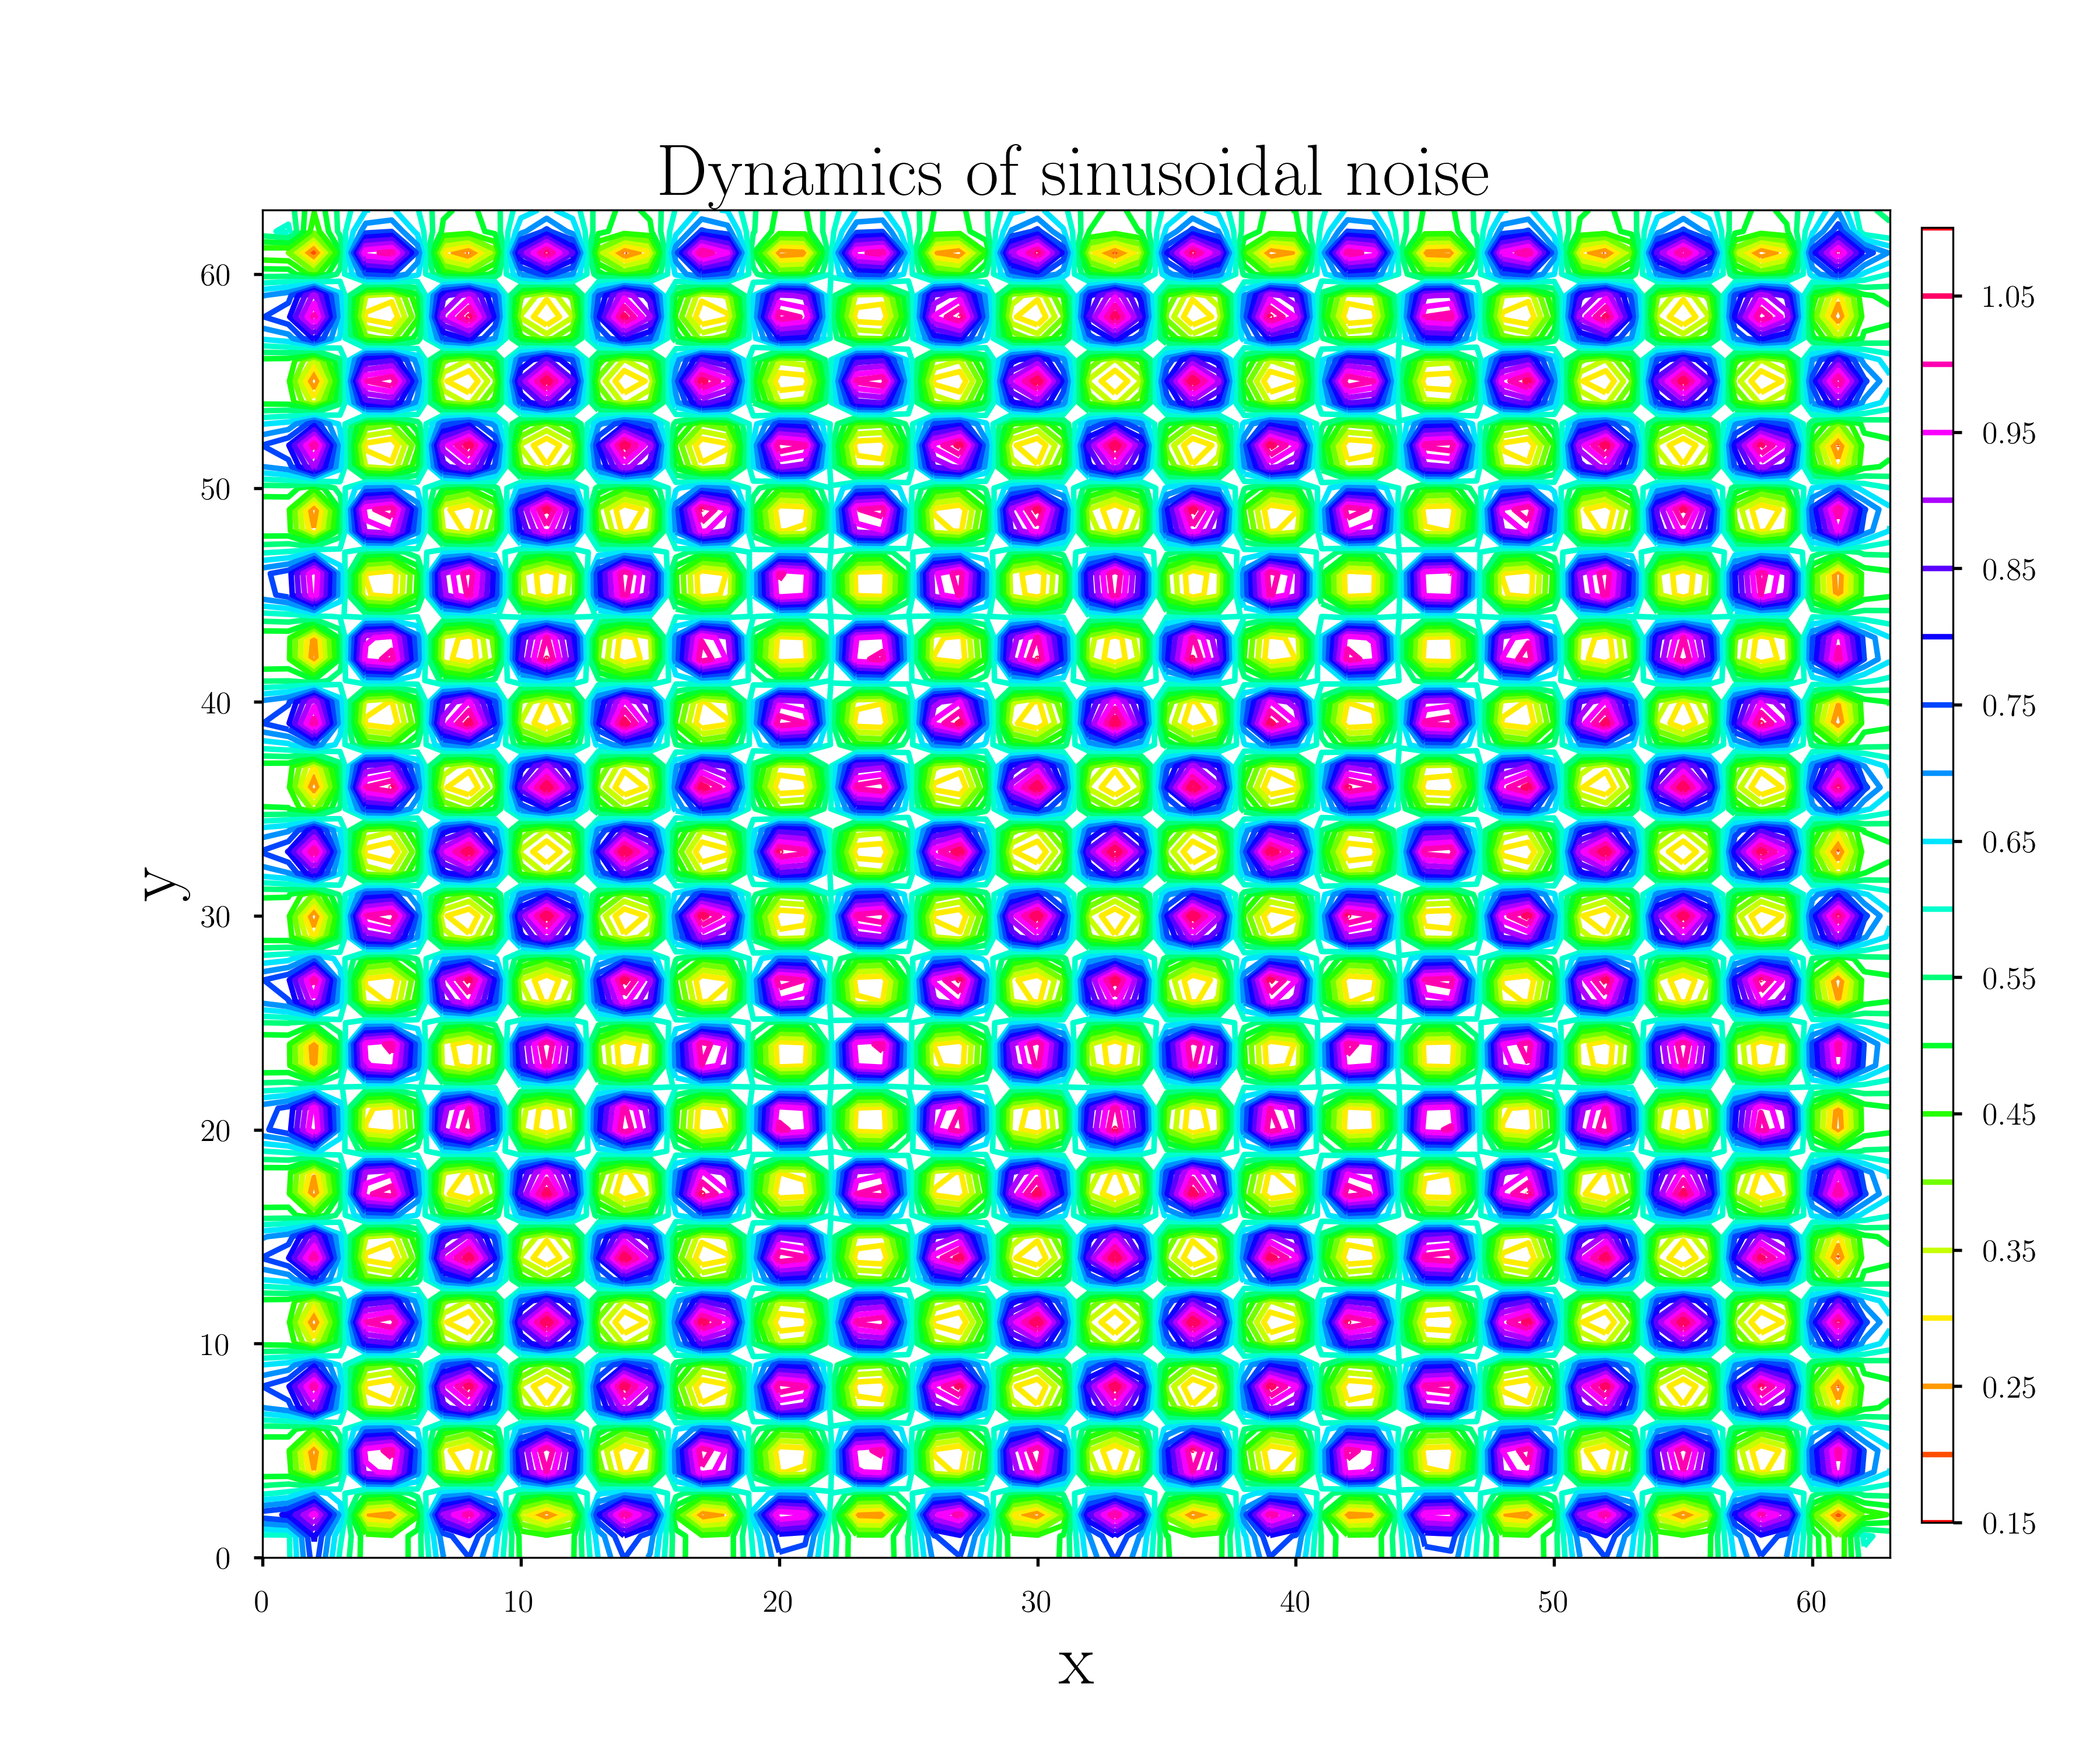
\includegraphics[width= \textwidth]{figures/sinus_noise_evol_100}
 	\subcaption{After $N_{\text{steps}} = 100$.}
 \end{subfigure}
 
 \caption{Evolution of a periodically perturbed density distribution}	
 \end{figure}